\chapter{Системийн шинжилгээ}
\section{Шаардлагууд}
\subsection{Хэрэглэгчийн шаардлага}

\begin{itemize}
  \item Хэрэглэгчийн алгоритм ба програмчлалын мэдлэгийг бататгаж, цааш өөр бодлогуудаар сорьдог байна.
  \item Хэрэглэгчид загвар код харуулж, бодох процессийг илүү хялбарчилсан байна.
  \item Програмчлалын үндсэн ойлголттой ямар ч хэрэглэгчид аппликейшн нь хэрэглэхэд ойлгомжтой, хүртээмжтэй интерфейстэй байна.
  \item  Хэрэглэгч өөрт тохирох дизайныг сонгож, customize хийх боломжтой байна.
  \item Хэрэглэгчид зориулсан editor нь хэрэглэгчийг бичиж байх үйл явцыг сонсон хурдан хариу өгөх intellisense-тэй байна.
  \item Хэрэглэгч амжилттай бодлогоо бодсоноор бусдын кодын хэрэгжүүлэлт, шийдлүүдийг харах боломжтой байна.
  \item Програмчлалын Python, Javascript болон C/C++(\textit{optional}), JAVA(\textit{optional}) хэлнүүд дээр бодлогыг бодох боломжтой байх.
  \item Хэрэглэгч кодоо ажиллуулах үед тэнцсэн эсвэл тэнцээгүй эсэхийг нь хэрэглэгчид мэдэгддэг байх ёстой.
  \item Систем нь монгол хэл бүхий хэрэглэгчийн интерфейстэй байх ёстой.
\end{itemize}

\subsection{Системийн шаардлага}
\begin{itemize}
  \item Сервер лүү brute-force байдлаар халдалт хийхээс сэргийлсэн байх.
  \item Өгөгдлийн сан руу хэрэглэгчид зөвхөн сервисүүдээр дамжин хандалт хийж болдог байх.
  \item Систем нь 24/7 ажиллагаатай байх бөгөөд хэзээ ч, хаанаас ч хандах боломжтой байна.
  \item  Бодлогын сан нь дахин сэргээх боломжтойгоор гараар backup хийдэг байна.
  \item Ачаалал даах чадвартай байх бөгөөд ямар нэгэн ачааллаас үүдэлтэй асуудал гарвал унтралгүйгээр тодорхой хугацааны дараа хэвийн ажиллагааг хангадаг байх.
  \item Хэрэглэгчээс оруулсан сэжиг бүхий кодууд compiler сервер дээр ажилладаггүй байна.
  \item Бодлого бүр тест кэйстэй байх шаардлагатай.
  \item Систем нь хэрэглэгчийн мэдээлэл болон бодсон бодлогуудын мэдээллийг хадгалдаг байх ёстой.
  \item Хэрэглэгчээс орж ирэх кодыг гуравдагч систем рүү хандах боломжгүй орчинд ажиллуулж үр дүнг гаргадаг байх хэрэгтэй.
\end{itemize}

\clearpage

\section{Технологийн асуудлууд}
"Coldbrains" систем нь програмчлалын бүтээгдэхүүн дотор програмчлалын үйл явцыг явуулж байгаа тул юун түрүүнд аюулгүй үйл ажиллагаа болон найдвартай байдлыг хангадах байх хэрэгтэй билээ. Нээлттэй вебсайтаар дамжуулан гадны ямар ч хэрэглэгч хэрэглэх боломжтой бөгөөд зохисгүй хэрэглэгчдийн үйл ажиллагааг хязгаарлах маш олон програмчлалын асуудлууд бий болж байна.

\subsection{Middleware}
Кодыг хүлээн авч ажиллуулж буй серверийг хэрэглэгчээс хязгаарлахын тулд тухайн хэрэглэгчийн веб аппликейшн болон серверийн хооронд middleware сервер байх бөгөөд энэхүү сервер нь хэрэглэгчээс ирэх хүсэлтүүдийг боловсруулан цааш дамжуулдаг байх шаардлагатай билээ. Үүнд:
\begin{itemize}
  \item Хэрэглэгчээс богино хугацаанд ирэх олон хүсэлтүүдийг хязгаарлах
  \item Жинхэнэ серверийн IP хаягийг нууцлан улмаар зөвхөн өөр дээрээсээ дамжуулах
  \item Хэрэглэгчийн эрхийг(user credentials/access token) шалгах
  \item Frontend-ээс ирэх Payload-ийг encrypt хийх
\end{itemize}
зэрэг үүргүүдийг гүйцэтгэх билээ.

\subsection{Sandboxing}
Middleware-ээр дамжуулагдан ирсэн кодыг аюулгүй эсвэл хортой код гэдгийг ялгах боломжгүй учраас тухайн кодны ажиллах орчныг зааж өгөн хязгаарлах шаардлагууд бий болсон. Үүнд:
\begin{itemize}
  \item Тухайн кодны үйл ажиллагаа нь ямарваа нэгэн байдлаар гадны гуравдагч endpoint руу хандах боломжгүй байх. Өөрөөр сүлжээнд нэвтрэх боломжгүй болгох. Тухайн програмчлалын хэлний ашиглагддаг built-in сүлжээнд холбогддог аргуудыг блоклох.
  \item Тухайн код нь үйлдлийн систем болон файл системд хандах боломжгүй байх. Хэрэв хандсан тохиолдолд тухайн үйлдлүүдийг хийсвэр орчинд гүйцэтгэх.
  \item Хэрэв код нь тухайн серверийн нөөцийг бүхэлд нь ашиглах тохиолдолд тухайн серверт нөөцийн хязгаарлалт бий болгох. Тухайн хязгаарыг давсан үед алдааг буцаадаг болгох.
  \item Хэрэглэгч бүрийн код бие даасан байдлаар ажилладаг байхын тулд серверүүдийг stateless\footnotemark{} \footnotetext{Төлөвгүй буюу ямарваа нэгэн байдлаар санах ойг шууд сав байдлаар ашигладаггүй байх} байдлаар зохиомжлох.
\end{itemize}
гэх мэт аюулгүй байдал болон зохиомжийн шийдлүүдийг боловсруулах шаардлагатай.

\subsection{Cloud үйлчилгээнүүд болон интеграц}
Дээр дурьдсан 2-т програм хангамж талаас асуудлуудыг тодорхойлсон бол эдгээр програм хангамжуудыг ажиллуулах техник хангамж, түүнийг ханган нийлүүлэгчдийг судалж үзэх нь дараачийн зайлшгүй асуудал мөн билээ. 

Програм хангамжуудыг stateless байдлаар хэрэгжүүлснээр тэдгээрт ашиглагдах бусад сервисүүдийн инстанцуудын ажиллагаа хязгаарлагдмал болдог билээ. Socket холбоо болон цаашлаад \textbf{singleton} загвараар хэрэгждэг холболтууд нь stateless байдлаар хэрэгжүүлэхэд зохимжгүй болдог. 

Үүнд ламбда илэрхийлэл буюу функциональ програмчлалын ойлголтуудыг зохиомж дээр хэрэгжүүлэх нь зүйтэй болно. Нарийвчилбал, өгөгдлийн сан, гуравдагч үйлчилгээ үзүүлэгчдийг 1 удаагийн холболтоор шийдэх арга замуудыг тодорхойлох асуудлууд гарч ирч буй юм.

\clearpage

\section{Ажлын явцын диаграм}
% \subsection{Ажлын явц(use case)-ын диаграм}

\begin{figure}[h]
  \centering
  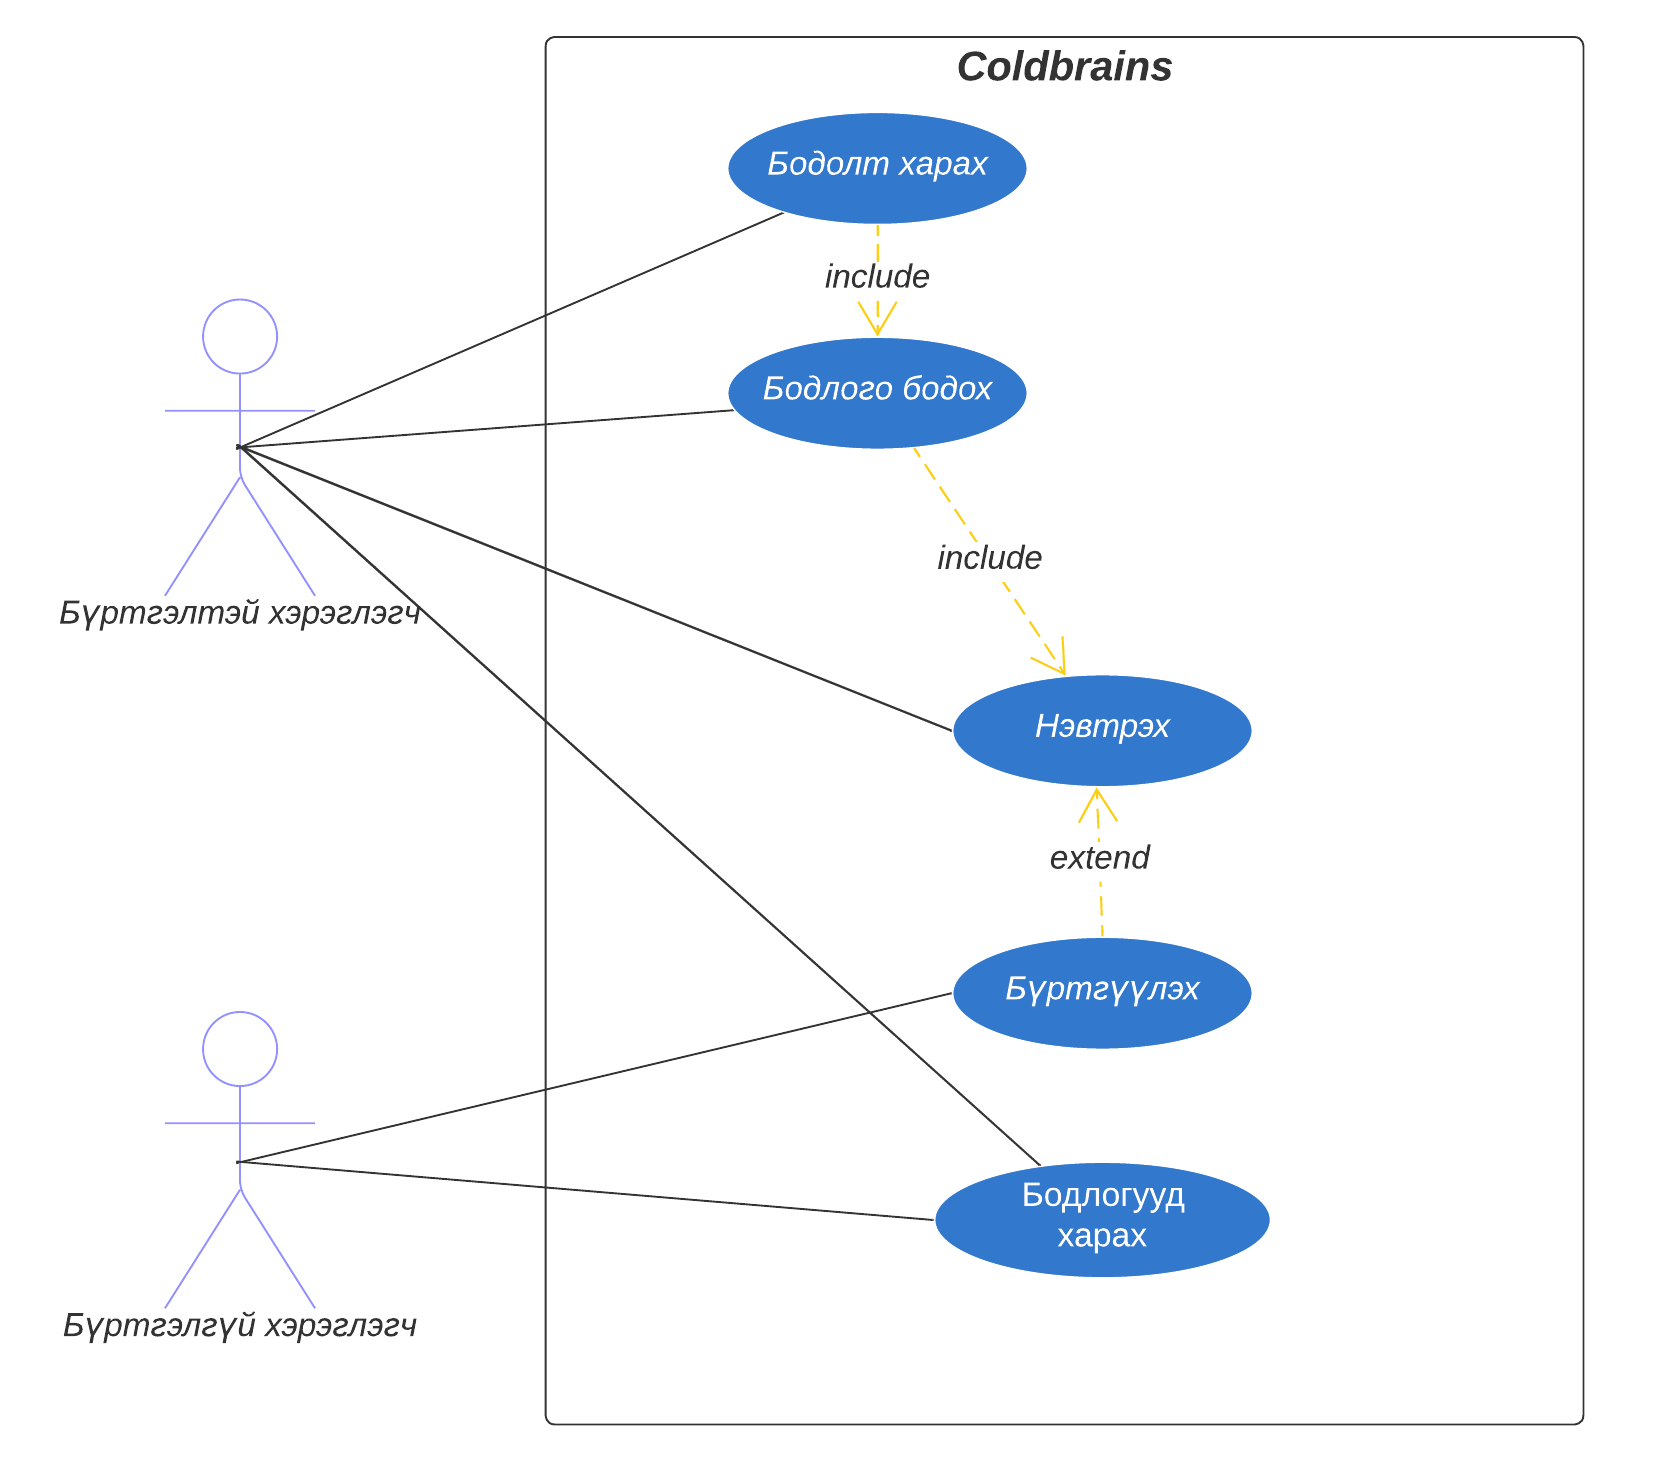
\includegraphics{img/diagrams/coldbrains-use-case.png}
  \caption{Ажлын явцын диаграм}
\end{figure}

Хэрэглэгчийг бүртгэлтэй болон бүртгэлгүй гэж ангилвал бүртгэлгүй хэрэглэгч нь системтэй танилцах зорилгоор бодлогуудын жагсаалтыг харах боломжтой бол бүртгэлтэй хэрэглэгч нь тухайн бодлогуудыг бодох, амжилттай бодсон бол бодолтуудыг харах, мөн өөрийн профайл хэсгийг харах боломжтой болно.

\clearpage

\textbf{Ажлын явц:} Бүртгүүлэх
\begin{table}[H]
  \begin{tabular}{|p{3cm}|p{13.5cm}|}
  \hline
  \multicolumn{1}{|c|}{Ажлын явц}                                       & \multicolumn{1}{c|}{Бүртгүүлэх}                                                                                                                                    \\ \hline
  Зорилго                                                                                       & Тоглогч системд бүртгэл үүсгэж нэвтрэхэд ашиглах                                                                                                                                           \\ \hline
  Угтвар нөхцөл                                                         & Тоглогч систем рүү хандсан байх                                                                                                                                                            \\ \hline
  Тоглогч                                                                                       & Coldbrains системд бүртгэлгүй хэрэглэгч   \\ \hline
  Тайлбарлалт                                                                                   & \begin{tabular}[c]{@{}l@{}}1. Систем нэр, нууц үг, и-мейл хаягийг шаардана.\\ 2. Шаардлагатай мэдээллийг оруулна.\\ 3. Систем амжилттай бүртгэн нэвтрэх хуудас луу шилжүүлнэ.\end{tabular} \\ \hline
  Өргөтгөл                                                                                      & Тоглогч буцах товч даран ажлын явцыг дуусгавар болгоно.                                                                                                                                    \\ \hline
  Хувилбар                                                                                      & 2a. Бүртгэлтэй хэрэглэгч байвал мэдэгдэж, мэдээллийг нь арилгана. Ажлын явцыг эхнээс нь эхлүүлнэ.                                                                                          \\ \hline
  \end{tabular}
\end{table}

\textbf{Ажлын явц:} Нэвтрэх
\begin{table}[H]
  \begin{tabular}{|p{3cm}|p{13.5cm}|}
  \hline
  \multicolumn{1}{|c|}{Ажлын явц}                                       & \multicolumn{1}{c|}{Нэвтрэх}                                                                                                                                    \\ \hline
  Зорилго                                                                                       & Тоглогч системийг ашиглахын тулд нэвтрэх                                                                                                            \\ \hline
  Угтвар нөхцөл                                                         & Тоглогч бодлогын тодорхойлолтыг харах, бодлого бодохыг оролдох,                                                                                                                                                   \\ \hline
  Тоглогч                                                                                       & Coldbrains системд бүртгэлтэй аль эсвэл шууд нэвтрэх сонирхолтой гадны платформд бүртгэлтэй хэрэглэгч                                                                                                                                                                                   \\ \hline
  Тайлбарлалт                                                                                   & \begin{tabular}[c]{@{}l@{}}1. Систем бүртгэлтэй нэр, нууц үг шаардана.\\ 2. Шаардлагатай мэдээллийг оруулна.\\ 3. Систем тоглогчид session үүсгэн бодлогууд хуудас руу шилжүүлнэ.\end{tabular} \\ \hline
  Өргөтгөл                                                                                      & Тоглогч буцах товч даран ажлын явцыг дуусгавар болгоно.                                                                                                                                    \\ \hline
  Хувилбар                                                                                      & 
  1a. Хэрэглэгч бусад платформуудын эрхийг оруулан session үүсгэж ажлын явцыг дуусгана.\newline 2a. Бүртгэлтэй хэрэглэгч олдоогүй бол мэдэгдэж, мэдээллийг нь арилгана. Ажлын явцыг эхнээс нь эхлүүлнэ.                                                                                          \\ \hline
  \end{tabular}
\end{table}

\clearpage

\textbf{Ажлын явц:} Бодлогууд харах
\begin{table}[H]
  \begin{tabular}{|p{3cm}|p{13.5cm}|}
  \hline
  \multicolumn{1}{|c|}{Ажлын явц}                                       & \multicolumn{1}{c|}{Бодлогууд харах}                                                                                                                                    \\ \hline
  Зорилго                                                                                       & Тоглогч системд буй бодлогын санг харах                                                                                                   \\ \hline
  Угтвар нөхцөл                                                         & Тоглогч систем рүү хандсан байх                                                                                                                                                   \\ \hline
  Тоглогч                                                                                       & Coldbrains систем рүү хандсан хэрэглэгч                                                                                                                                              \\ \hline
  Тайлбарлалт                                                                                   & \begin{tabular}[c]{@{}l@{}}1. Систем бодлогын санг хэрэглэгчид харуулна.\end{tabular} \\ \hline
  \end{tabular}
\end{table}

\textbf{Ажлын явц:} Бодолт харах
\begin{table}[H]
  \begin{tabular}{|p{3cm}|p{13.5cm}|}
  \hline
  \multicolumn{1}{|c|}{Ажлын явц}                                       & \multicolumn{1}{c|}{Бодолт харах}                                                                                                                                    \\ \hline
  Зорилго                                                                                       & Тоглогч бодсон бодолгынхоо аргуудаас суралцах зорилгоор бусдын бодолтуудыг харах                                                                                                       \\ \hline
  Угтвар нөхцөл                                                         & Тоглогч тухайн бодлогыг бодсон байх                                                                                                                                                   \\ \hline
  Тоглогч                                                                                       & Системд нэвтэрч орон session үүсгэсэн хэрэглэгч      \\ \hline
  Тайлбарлалт                                                                                   & \begin{tabular}[c]{@{}l@{}}1. Систем тухайн бодлогын бодолтуудыг өөрийн бодолтын хамт харуулна.\\ 2. Тухайн бодолтуудын ямар хэл болон ажилласан хугацааг харуулна.\end{tabular} \\ \hline
  \end{tabular}
\end{table}

\clearpage

\textbf{Ажлын явц:} Бодлого бодох
\begin{table}[H]
  \begin{tabular}{|p{3cm}|p{13.5cm}|}
  \hline
  \multicolumn{1}{|c|}{Ажлын явц}                                       & \multicolumn{1}{c|}{Бодлого бодох}                                                                                                                                    \\ \hline
  Зорилго                                                                                       & Тоглогч системийн бодлогын сангаас бодлого сонгож бодон тухайн бодлогын талаар суралцах, бусдаас шийдлүүдийг сурч авах                                                              \\ \hline
  Угтвар нөхцөл                                                         & Системд нэвтэрч орон бодлогоо сонгосон байх.  \\ \hline
  Тоглогч                                                                                       & Системд нэвтэрч орон session үүсгэсэн хэрэглэгч                            \\ \hline
  Тайлбарлалт                                                                                   & \begin{tabular}[c]{@{}l@{}}1. Систем хэрэглэгчид бодлогын тодорхой тайлбар болон жишээ оролт\\ болон гаралтыг харуулна.\\ 2. Систем оролтод ашиглах boilerplate\footnotemark{} код бүхий код засварлагчийг\\ үүсгэж өгнө.\\ 3. Тоглогч тухайн бодлогын бодолт бүхий кодыг бичнэ.\\ 4. Тоглогч тухайн кодыг ажиллуулах товчийг дарна.\\ 5. Тоглогч тухайн бодлогын бодолтууд хуудас руу шилжинэ.\end{tabular} \\ \hline
  Өргөтгөл & 4b. Тоглогч кодоо дахин засварлаж дараагийн алхмаа хийнэ.\newline 2a. Тоглогч өөрийн дуртай код засварлагчийн загваруудаас сонгоно. \newline 1b. Тоглогч өөрийн мэддэг програмчлалын хэлээ сонгоно.   \\ \hline
  Хувилбар                                                                                      & 
  4a. Тоглогчийн кодын алдааны мэдээлэл болон харгалзах тест кейсийг систем харуулан ажлын явц үргэлжлэнэ.                                                                    \\ \hline
  \end{tabular}
\end{table}
\footnotetext{Ерөнхий хүрээнд ашиглах боломжтой, өөрчлөлт оруулж болох бүхий код}